%% CSD Assignment 1 - Final Technical Report
%% Uses the supplied ACM manuscript template without changing its layout.
\documentclass[manuscript,screen,review]{acmart}
\usepackage{xurl}
\hypersetup{colorlinks=true,linkcolor=black,citecolor=black,urlcolor=blue}

\AtBeginDocument{\providecommand\BibTeX{{Bib\TeX}}}
\setcopyright{none}
\settopmatter{printacmref=false,printfolios=true}
\renewcommand\footnotetextcopyrightpermission[1]{}

\begin{document}

\title{Web-Based Village Pond Planning System}
\subtitle{CSD Assignment 1 -- Phase 3 Final Technical Report}

\author{Sneha Nagmoti}
\affiliation{%
  \institution{Indian Institute of Technology Bhilai}
  \city{Durg}
  \country{India}}
\email{snehan@iitbhilai.ac.in}
\renewcommand{\shortauthors}{Nagmoti}

\begin{abstract}
This report presents a web-based decision-support system for preliminary village pond planning. A user can select a study centre and radius on an interactive satellite map, or upload surveyed contour geometry in KML/KMZ form. The backend reconstructs a terrain surface, removes artificial depressions with Priority-Flood, resolves flats, computes D8 flow direction and accumulation, delineates the contributing watershed, and ranks spatially separated pond candidates. Satellite colour screening excludes detected surface water and identifies candidate open land. Historical rainfall is aggregated from complete calendar years; annual runoff is estimated by $V=C(P/1000)A$, with rainfall $P$ in millimetres and area $A$ in square metres. A geometry model converts usable runoff into pond depth, capacity, footprint and excavation dimensions while enforcing side-slope, freeboard and land-area limits. Results are returned as structured JSON and visualized as map overlays. In the verified live example, the system reported a 119.01 ha catchment, 1,324.2 mm annual rainfall, 472,758 m$^3$/year runoff and three ranked sites; the selected design stores 378,206 m$^3$. The delivered implementation includes a responsive React/Leaflet interface, a documented FastAPI service, public-data fallbacks, validation and rate limits, and automated backend and frontend tests.
\end{abstract}

\keywords{Village Pond Planning, Geospatial Analysis, Rainwater Harvesting,
  Catchment Estimation, Web GIS, REST APIs}

\maketitle

\section{Introduction}
Seasonal rainfall can provide substantial local storage, but selecting a pond site is difficult because elevation, drainage, land cover and rainfall must be interpreted together. A site chosen only from a visual map can fall on a ridge, intercept little contributing area, overlap water, or require impractical excavation. The project therefore implements a geospatial web application that turns a selected land area or uploaded contour map into auditable pond-planning evidence. It produces a suggested site, watershed boundary, rainfall statistic, expected runoff, pond volume and dimensions, and renders these results directly on the map. The following sections define the requirements, architecture, hydrological method, implementation, CSD decisions and measured results.

\subsection{Motivation}
Manual screening is slow and inconsistent: contour interpretation is specialist work, rainfall records are distributed across services, and current land or surface-water conditions are not obvious from coordinates alone. Combining these inputs in one repeatable pipeline helps an administrator compare alternatives before commissioning a field survey. The tool is deliberately a screening system: it makes the data and assumptions visible instead of replacing engineering approval.

\subsection{Scope of the Project}
The system (i) supports map-based centre/radius selection and KML/KMZ contour upload; (ii) reconstructs terrain and drainage; (iii) identifies up to three ranked, separated pond options outside detected water; (iv) estimates catchment area, annual rainfall, runoff, storage capacity and excavation geometry; and (v) visualizes the watershed, candidates, elevation and drainage evidence. It does not certify land ownership, soil permeability, dam stability, flood safety or construction drawings. Final selection therefore requires cadastral, hydrographic, geotechnical and field verification.

\section{Problem Statement and Requirements}
The required system must accept a user-defined land area, analyze its terrain and rainfall, recommend a pond site, and display the site, catchment and expected water volume on a usable frontend. Table~\ref{tab:requirements} maps each requirement to the implemented component.

\begin{table}[h]
  \caption{Functional requirements and implementation}
  \label{tab:requirements}
  \begin{tabular}{p{3.7cm}p{4.8cm}}
    \toprule
    Requirement & Implemented in \\
    \midrule
    Satellite map and land selection & React/Leaflet map, search, coordinate and radius controls \\
    Contour visualization/upload & Upload workspace and \texttt{/api/analyze-contour} \\
    Candidate-land identification & RGB/HSV OpenCV screening with morphology and water mask \\
    Catchment estimation & Priority-Flood, resolved-flat D8 and reverse watershed traversal \\
    Historical rainfall & Open-Meteo archive with NASA POWER fallback \\
    Runoff and pond sizing & \texttt{terrain.py} volumetric runoff and trapezoidal geometry \\
    Combined result view & Toggleable Leaflet layers, ranked markers and result cards \\
    Structured API output & Validated Pydantic response models and Swagger/ReDoc \\
    \bottomrule
  \end{tabular}
\end{table}

\subsection{Non-Functional Requirements}
The application is responsive on current desktop and mobile browsers and keeps analysis work asynchronous so external calls do not freeze the interface. The API validates coordinate, radius, upload type, archive contents and size; applies per-route rate limits; restricts trusted hosts/CORS; and returns explicit source-quality metadata. The backend is stateless when optional history is disabled, so identical replicas can be placed on the four allotted systems. External failures use bounded timeouts, retries, cache and documented fallbacks rather than fabricated values. The production frontend is a static bundle, while health endpoints support availability checks. Target interaction latency is seconds for live screening and under one minute for a 15 MiB contour upload.

\section{System Architecture and High-Level Design}
The browser collects a location/radius or multipart contour file and calls the FastAPI service over HTTPS. Independent asynchronous adapters obtain elevation, satellite imagery and historical rainfall. The terrain and vision services normalize those inputs, the hydrology service computes drainage and candidates, and a sizing service produces runoff and pond geometry. Typed response models return both values and map geometry. Optional SQLite history is isolated from analysis and is disabled in the public demo; cache entries reduce repeated public-API calls. Figure~\ref{fig:architecture} shows this flow.

\begin{figure}[h]
  \centering
  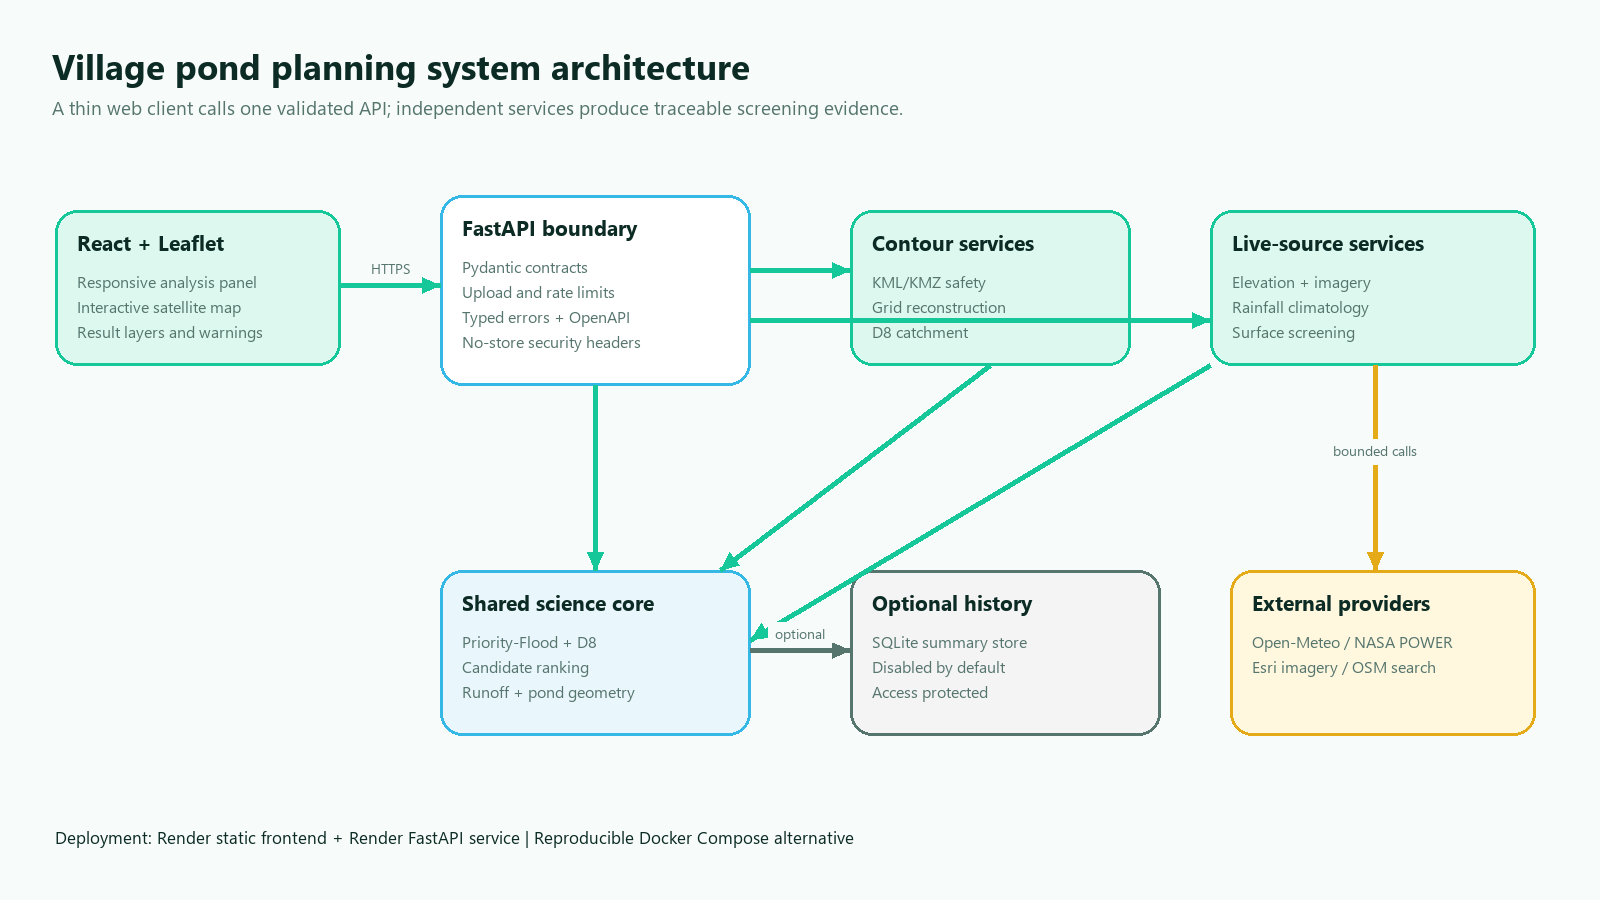
\includegraphics[width=0.96\linewidth]{architecture.png}
  \caption{High-level client, API, analysis-service and public-data architecture.}
  \label{fig:architecture}
  \Description{A React and Leaflet client calls a FastAPI backend whose terrain, imagery, rainfall and contour services produce analysis results and optional cached history.}
\end{figure}

\subsection{Technology Stack}
The frontend uses React, Vite and Leaflet. The backend uses Python, FastAPI, Pydantic, NumPy, SciPy, OpenCV, Rasterio, Shapely, GeoPandas and HTTPX. Elevation comes from Open-Meteo/Copernicus GLO-90 compatible data with a bounded tile fallback; rainfall uses Open-Meteo Archive and NASA POWER; Esri World Imagery supplies the displayed and analyzed satellite mosaic. SQLite/SQLAlchemy provides optional local history. Pytest and Vitest test the two layers, and Docker/Render configurations provide reproducible deployment. This stack was chosen because its geospatial libraries implement the required raster/vector operations while FastAPI exposes an inspectable JSON contract.

\section{Methodology}
Both input modes enter the same hydrological core. Live mode samples an elevation grid over the chosen radius. Contour mode parses KML/KMZ safely, extracts line elevations, projects coordinates to metric space, rasterizes observations and performs fixed-observation harmonic interpolation. The latter iteratively replaces unobserved cells by neighboring means while never changing contour cells; convergence and observed-cell ratio are reported in the response.

\subsection{Terrain and Elevation Analysis}
The DEM is depression-filled with Priority-Flood so isolated numerical pits do not trap all flow. A small deterministic gradient resolves equal-height flats. Each valid cell then selects its steepest lower neighbour among the eight adjacent cells (D8). Processing cells in topological order gives flow accumulation in $O(n)$ after the $O(n\log n)$ flood, where $n$ is the number of grid cells. Contours displayed by the frontend are regenerated from this surface. For uploaded data the original contour lines remain visible, making interpolation and source coverage auditable.

\subsection{Catchment Area Delineation and Site Ranking}
Candidate cells must lie inside the study/candidate-land mask, outside detected water and its buffer, away from the analysis boundary, and on a routable cell. A weighted score favors high log-flow accumulation (0.52--0.58 weight), low elevation, low local slope, interior clearance and distance from detected water. Non-maximum spatial separation prevents the top three options from collapsing onto the same point. For a chosen candidate, reverse traversal follows every D8 link that drains to it; the number of upstream cells multiplied by projected cell area gives the contributing area. Thus the reported catchment belongs to the selected pond point rather than to an unrelated study-area outlet. The drainage path is traced downstream for visual inspection.

\subsection{Rainfall, Runoff and Pond Geometry}
Daily precipitation is grouped into complete calendar years; incomplete years are excluded before computing mean annual rainfall. If the primary archive is unavailable, NASA POWER is queried with the same completeness checks. Annual runoff is
\begin{equation}
  V=C\left(\frac{P}{1000}\right)A,
\end{equation}
where $A$ is catchment area in m$^2$, $P$ is annual rainfall in mm, and the course-demo coefficient is $C=0.30$. The coefficient and its source are returned explicitly. A configurable capture fraction converts runoff to target storage. Pond length, width and water depth are solved for a rectangular basin with 2H:1V side slopes and 0.5 m freeboard; dimensions are reduced if the detected candidate land cannot contain the excavation footprint.

\section{Implementation}
\subsection{Backend and API Design}
The main routes are summarized in Table~\ref{tab:endpoints}. The upload route accepts either \texttt{contour\_file} or the assignment-compatible \texttt{contour\_map} field; \texttt{/api/analyzeContour} and \texttt{/api/findCatchment} remain compatibility aliases. Validation errors use 4xx responses; third-party failures are bounded, recorded per source, and either fall back or produce an incomplete result instead of a false success. No login is needed for the public screening demo; history, when enabled, requires its configured access control.

\begin{table}[h]
  \caption{Public API endpoints}
  \label{tab:endpoints}
  \begin{tabular}{p{2.0cm}p{4.1cm}p{2.5cm}}
    \toprule
    Method & Path & Purpose \\
    \midrule
    POST & \texttt{/api/analyze} & Location/radius analysis \\
    POST & \texttt{/api/analyze-contour} & KML/KMZ terrain analysis \\
    GET & \texttt{/api/search-village} & Submitted place search \\
    GET & \texttt{/health/live}, \texttt{/health/ready} & Service checks \\
    GET & \texttt{/docs}, \texttt{/redoc} & API documentation \\
    \bottomrule
  \end{tabular}
\end{table}

\subsection{Frontend and Visualization}
The interface offers Live Analysis and Contour Upload workspaces. A collapsible result panel leaves the map available for inspection. Users can select a location by search, coordinates or map interaction, set the radius, upload KML/KMZ, choose automatic/point/region contour selection, and switch among ranked options. Leaflet overlays show the study radius, source contours, reconstructed elevation surface, candidate land, water exclusion, catchment boundary, drainage path and numbered pond sites. Result cards present catchment, rainfall, runoff, capacity, depth, dimensions, score and source status in plain language. Figure~\ref{fig:ui} shows the verified live result.

\begin{figure}[h]
  \centering
  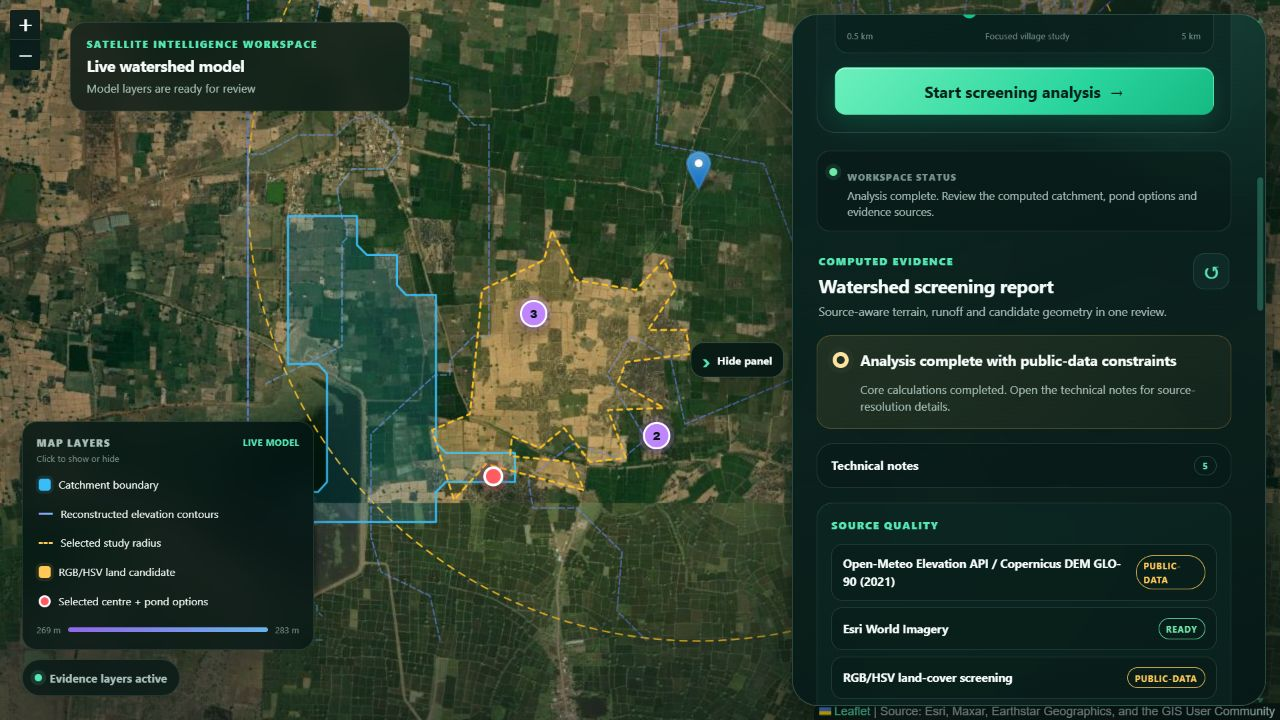
\includegraphics[width=0.98\linewidth]{live-results.png}
  \caption{Deployed live-analysis interface with catchment, candidate land and ranked sites.}
  \label{fig:ui}
  \Description{Satellite map with a blue watershed, yellow candidate land, three numbered pond options and a source-aware result panel.}
\end{figure}

\subsection{Database and Storage}
Analysis responses are self-contained and do not depend on persistence. A small SQLite store can retain selected summary records for a protected history view, but public deployment disables history to minimize stored user data. Public-source responses use bounded local caches with expiry; uploaded archives are processed in memory/temporary storage and are not used as permanent data.

\section{CSD Themes and Topics Applied in the Project}
\begin{table}[h]
  \caption{CSD concepts and concrete use}
  \label{tab:csd-themes}
  \begin{tabular}{p{2.4cm}p{5.9cm}}
    \toprule
    Theme & Application and rationale \\
    \midrule
    REST contracts & Versionable typed requests/responses separate UI from analysis. \\
    Concurrency & Elevation, imagery and rainfall are awaited concurrently to reduce wall time. \\
    Caching & Repeated public-data queries reuse bounded TTL entries, reducing latency and quotas. \\
    Modularity & Source adapters and hydrology/vision services can be replaced independently. \\
    Resilience & Timeouts, retries, fallbacks and quality states expose partial-source failures. \\
    Security & Upload/archive validation, limits, CORS, trusted-host and rate controls reduce attack surface. \\
    Scalability & Stateless analysis and a static frontend allow independent replication on allotted hosts. \\
    Testing/CI & Unit, integration and UI tests verify algorithms, contracts and Nginx security headers. \\
    \bottomrule
  \end{tabular}
\end{table}

The most important decision was a modular monolith rather than premature microservices: geospatial arrays remain in one process, avoiding serialization overhead, while source clients and algorithms still have clean interfaces. Asynchronous public-data calls shorten the critical path, while CPU-heavy terrain work remains deterministic and testable. Quality metadata is treated as part of the API contract; a successful HTTP call cannot silently turn missing rainfall or land evidence into a precise engineering answer. Because analysis is stateless, the same container can be replicated across the four laboratory systems and placed behind a reverse proxy if concurrency requires it.

\section{Results and Evaluation}
The deployed live workflow was manually verified at 21.244025$^\circ$N, 81.288000$^\circ$E. It produced three pond alternatives and the representative values in Table~\ref{tab:results}. The selected design stores 80\% of annual modeled runoff and respects the configured depth, side-slope and footprint constraints. The supplied \texttt{contours\_1m.kml} was also processed generically: 1,355 contours and 159,113 source points formed a 148$\times$181 grid with 18 m cells; 85.206\% of grid cells were directly observed and harmonic interpolation converged in 31 iterations. Its coloured DEM and ranked sites are shown in Figure~\ref{fig:results}. These are model-derived screening results, so correctness is evaluated by invariants, source traceability and map coherence rather than unavailable field ground truth.

\begin{table}[h]
  \caption{Representative live-analysis result}
  \label{tab:results}
  \begin{tabular}{p{4.4cm}r}
    \toprule
    Measure & Result \\
    \midrule
    Catchment area & 119.01 ha \\
    Mean annual rainfall & 1,324.2 mm/year \\
    Expected runoff ($C=0.30$) & 472,758 m$^3$/year \\
    Suggested pond location & 21.250558, 81.296762 \\
    Suitability score & 96.2 / 100 \\
    Water storage capacity & 378,206 m$^3$ \\
    Water/excavation depth & 4.0 / 4.5 m \\
    Water dimensions & 382.57 $\times$ 260.38 m \\
    Excavation footprint & 100,901 m$^2$ \\
    \bottomrule
  \end{tabular}
\end{table}

\begin{figure}[h]
  \centering
  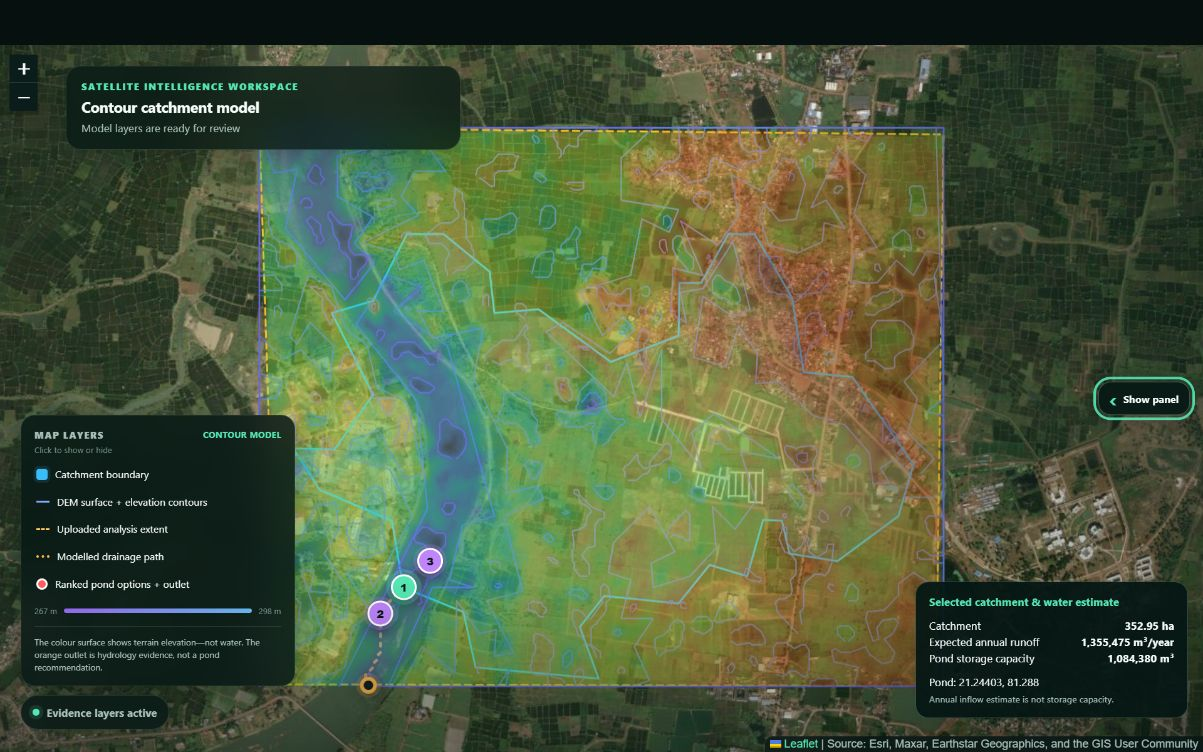
\includegraphics[width=0.98\linewidth]{contour-final-desktop.png}
  \caption{Fresh allotted-system contour result: coloured DEM, catchment, drainage path and three ranked options, with 352.95 ha catchment, 1,355,475 m$^3$/year runoff and 1,084,380 m$^3$ storage displayed on the map.}
  \label{fig:results}
  \Description{A coloured interpolated elevation surface on satellite imagery with contour lines, a catchment boundary, drainage path and three ranked candidate markers.}
\end{figure}

\subsection{Performance and Verification}
\begin{figure}[h]
  \centering
  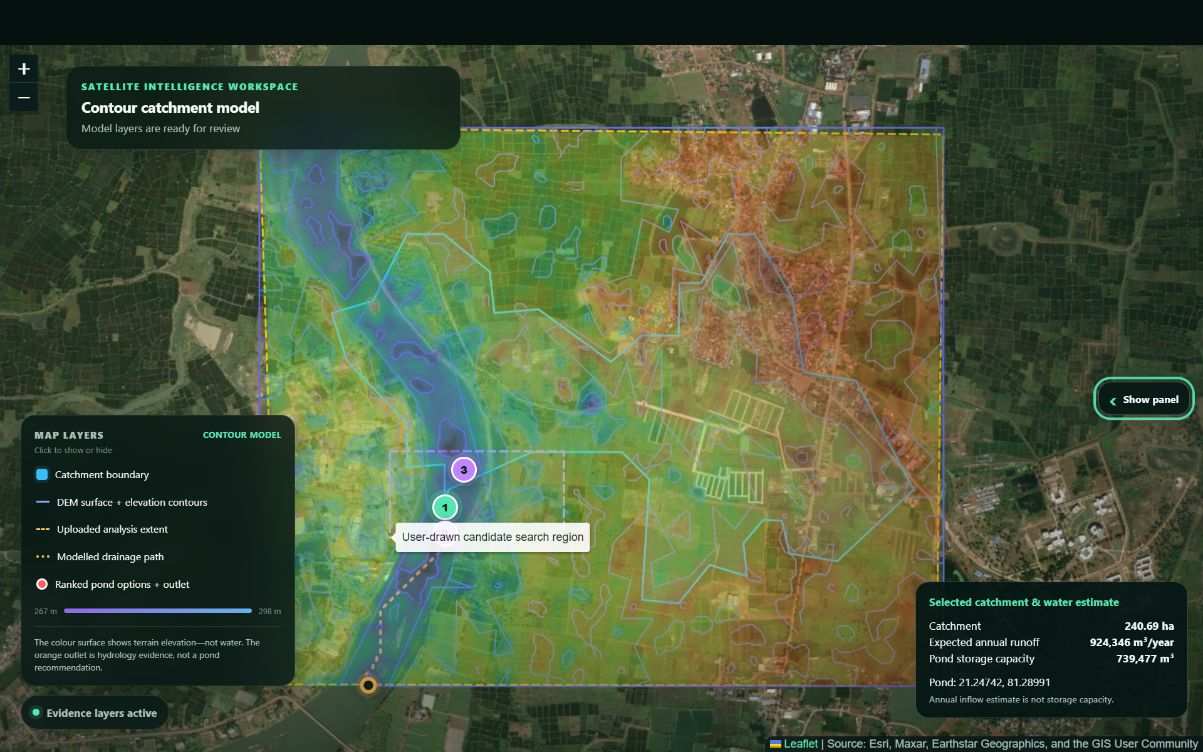
\includegraphics[width=0.68\linewidth]{region-final-desktop.png}\hfill
  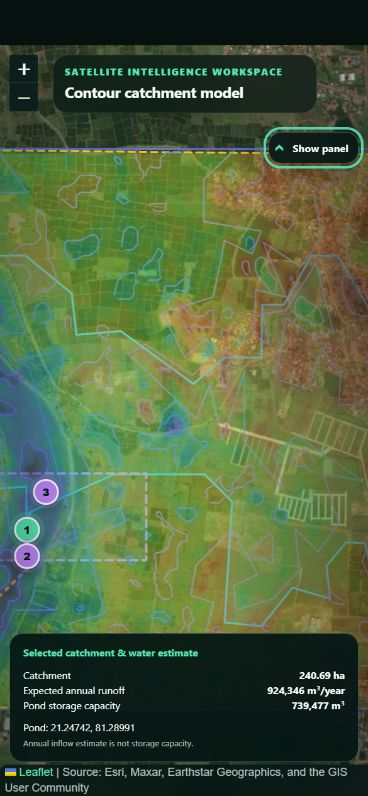
\includegraphics[width=0.27\linewidth]{region-final-mobile.png}
  \caption{User-drawn search region after recomputation, shown at desktop and mobile widths. The changed site has 240.69 ha catchment, 924,346 m$^3$/year runoff and 739,477 m$^3$ proposed storage. The dashed search polygon restricts pond placement, not the full upstream catchment.}
  \Description{Desktop and mobile screenshots of the same selected-region analysis, showing the search polygon, three candidate markers, catchment boundary and numerical map summary.}
\end{figure}
Tests cover Priority-Flood/D8 behavior, independent reference-walk checks of flow accumulation and catchment membership, point/region selection, water exclusion, contour parsing, upload limits, source failures, runoff/geometry constraints and map-result presentation. In the 26 September baseline, a full supplied-contour request through the college HTTP endpoint completed in 31.58 s. A cold live request lacked imagery and withheld a recommendation; a subsequent run completed with three candidates. These are functional and numerical-consistency checks, not validation against a surveyed watershed.

On the allotted container's 512 MiB memory and one-CPU quota, two simultaneous supplied-KML requests completed successfully in 41.38 s and 59.05 s. Both produced the same 3,529,523.47 m$^2$ catchment and 1,355,474.66 m$^3$/year runoff; an independent multiplication of area, rainfall and coefficient agreed with the reported volume. All 15 concurrent readiness probes succeeded, with a maximum response time of 0.271 s. This bounded concurrency test supports a small demonstration workload; it is not a sustained saturation benchmark or a high-availability claim.

\paragraph{Repeated submission checks (27 September 2026).}
All 76 backend tests passed again locally (24.10 s) and on system 2 (33.84 s). All 14 frontend tests, both linters and the production build passed. Manual testing exposed a retry-selection bug: failed candidate requests could revert to the preceding selection. The fix preserves the requested mode and point, and routes retries by workflow; regression checks cover both cases. The real API accepted equivalent KML/KMZ, recomputed a point and region, and returned HTTP 422 for malformed files, wrong upload fields, invalid latitude and out-of-coverage points. Browser checks covered coordinate validation, upload, layer/panel toggles, a four-vertex region with changed results and a 390-pixel layout without horizontal overflow. Connection failures required retries. A live run lacked imagery; a later contour run applied the 60 m water buffer. Failed attempts are not complete passes, and earlier live results do not guarantee upstream availability.

\subsection{Allotted-System Deployment and Recovery}
The frontend and API run together on allotted system 2, accessed through SSH port 2238. External HTTP port 3238 forwards to its internal port 3000. The frontend uses relative \texttt{/api} requests, so the demonstration does not depend on the Render backend. User-owned Supervisor restarts an exited application process; this recovery was verified. A container reboot requires the documented start command because the container's initial process is SSH rather than a service manager. Successful satellite tiles are cached with a bounded lifetime, allowing missing-tile retries without accepting partial imagery. Intermittent college-network and upstream connection failures remain possible; source failures are shown explicitly.

The map displays the selected catchment boundary and pond options, with an on-map summary of catchment area, expected annual runoff, coordinates and storage capacity. Annual collected runoff and physical storage capacity are labelled separately. On narrow screens the summary remains visible with the controls panel collapsed. Deployment commands, resource checks and reproducible verification scripts are included in the repository.

\section{Discussion and Limitations}
The strongest result is traceability: every recommendation is accompanied by its watershed, ranked alternatives, source states and assumptions. Nevertheless, GLO-90-scale/public elevation cannot resolve small bunds and culverts; harmonic reconstruction between contours smooths unmeasured terrain; RGB/HSV screening may miss narrow, muddy, shaded or seasonal water; a uniform runoff coefficient ignores soil and land-use variation; and long-term annual rainfall does not replace design-storm routing. Land ownership is not inferred. The map therefore supports comparative screening, not construction approval. Future work should incorporate verified cadastral parcels, higher-resolution survey DEMs, official hydrography, soil-specific coefficients, IDF curves, spillway routing and measured validation sites.

\section{Submission Links}
\begin{table}[h]
  \caption{Clickable submission and verification links}
  \label{tab:submission-links}
  \begin{tabular}{p{2.7cm}p{5.6cm}}
    \toprule
    Item & Link \\
    \midrule
    GitHub repository & \href{https://github.com/snehanagmoti/Village-Pond-planning}{Open source repository} \\
    Public demo video & \href{https://youtu.be/Kt8YKtDSnM0}{Watch the five-minute demonstration} \\
    Public frontend & \href{https://sneha-village-pond-planning-2026.onrender.com/}{Open public web application} \\
    Allotted-system frontend & \href{http://10.1.75.53:3238/}{Open college-system application} \\
    Interactive API docs & \href{http://10.1.75.53:3238/docs}{Open Swagger documentation} \\
    Contour-analysis API & \href{http://10.1.75.53:3238/api/analyze-contour}{POST /api/analyze-contour} (field: \texttt{contour\_map}) \\
    \bottomrule
  \end{tabular}
\end{table}
The allotted-system URLs require access to the college network. The public demonstration video and Render frontend remain accessible outside that network.

\section{AI-Assistance Disclosure}
AI tools were used for reviewing code and for report formatting. All technical statements were checked against the source code, automated test results, deployed API responses and map output. AI output was not used as hydrological ground truth; terrain, catchment and runoff results are produced by the implemented algorithms from the stated inputs and assumptions.

\begin{thebibliography}{6}
\bibitem{openmeteo} Open-Meteo, ``Historical Weather and Elevation APIs,'' \url{https://open-meteo.com/}.
\bibitem{nasa} NASA POWER Project, ``Daily Meteorology API,'' \url{https://power.larc.nasa.gov/}.
\bibitem{copernicus} Copernicus Programme, ``Copernicus DEM GLO-90,'' European Space Agency.
\bibitem{leaflet} Leaflet, ``An open-source JavaScript library for mobile-friendly interactive maps,'' \url{https://leafletjs.com/}.
\bibitem{fastapi} FastAPI, ``FastAPI framework documentation,'' \url{https://fastapi.tiangolo.com/}.
\bibitem{priorityflood} R. Barnes, C. Lehman, and D. Mulla, ``Priority-Flood: An optimal depression-filling and watershed-labeling algorithm for digital elevation models,'' \emph{Computers \& Geosciences}, vol. 62, pp. 117--127, 2014.
\end{thebibliography}

\end{document}
\endinput
